\documentclass[dvipsnames, notes]{beamer}

\usetheme{Warsaw}

\usepackage{inputenc}
\usepackage{amsmath}
\usepackage{amsthm}
\usepackage{graphicx}
%\usepackage{geometry}
\usepackage{tasks}
\ifodd\textwidth
  \addtolength{\textwidth}{1sp}
\fi

\newcommand{\po}{\textcolor{BlueViolet}{po}}
\newcommand{\ppo}{\textcolor{BlueViolet}{ppo}}
\newcommand{\rf}{\textcolor{Green}{rf}}
\newcommand{\rfe}{\textcolor{Green}{rfe}}
\newcommand{\ws}{\textcolor{BurntOrange}{ws}}
\newcommand{\fr}{\textcolor{RubineRed}{fr}}
\newcommand{\com}{\textcolor{BurntOrange}{com}}
\newcommand{\barr}{\textcolor{Apricot}{bar}}

\newcommand{\ghb}{\textcolor{NavyBlue}{ghb}}

\newcommand{\ato}{\textcolor{RoyalPurple}{ato}}


\newcommand{\co}{\textcolor{BurntOrange}{co}}
\newcommand{\mo}{\textcolor{Red}{mo}}
\newcommand{\hbsc}{\textcolor{NavyBlue}{hbsc}}
\newcommand{\xhb}{\textcolor{NavyBlue}{xhb}}
\newcommand{\rfi}{\textcolor{Green}{rfi}}
\newcommand{\brf}{\textcolor{Green}{brf}}
\newcommand{\jhb}{\textcolor{NavyBlue}{jhb}}
\newcommand{\jmo}{\textcolor{Red}{jmo}}

\title{Making Weak Memory Models Fair}
\subtitle{Ori Lahav, Egor Namakanov, Jonas Oberhauser, Anton Podkopaev, Viktor Vafeiadis}

\author{Presented by \\ Akshay Gopalakrishnan}

\begin{document}

    \begin{frame}

        \maketitle

    \end{frame}

    \begin{frame}{Introduction}

      \begin{itemize}
        \item Termination guarantees in a concurrent environment relies on fairness.
        \item In particular, thread-fairness, which ensures that each thread is eventually scheduled to run each instruction till the end.
        \item While this is sufficient for interleaving semantics (Sequential consistency), thread-fairness is not sufficient for weaker models of concurrency. 
        \item The key problem lies behind the lack of write propagation guarantee from one thread to another under weaker models.
        \item The additional constraint required is termed as memory-fairness, which in conjunction with thread-fairness can be used to reason about program termination under weak memory models.
      \end{itemize}
      
    \end{frame}

    \begin{frame}{Paper's Contributions}

      \begin{itemize}
        \item Identifies memory fairness guarantees for Operational and Declarative style models of concurrency.
        \item In particular, fairness constraints for $SC, TSO, RA, StrongCOH$ were identified.
        \item Equivalence between both operational and declarative memory fairness constraints were proven. 
        \item Above results were extended to identify memory fairness for $RC11$, showcasing that existing results over compilation and correctness of optimizations remain unchanged.
      \end{itemize}
      
    \end{frame}

    \begin{frame}{Example Spinlock}

      \begin{figure}
        \makebox[\textwidth][c]{
            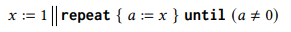
\includegraphics{INF_LOOP_EX1.png}
      }
      \end{figure}

      \begin{itemize}
        \item The loop will not terminate until the corresponding loop thread in scheduled.
        \item The loop will not terminate until the corresponding thread modifying the value of $x$ is scheduled.
      \end{itemize}
      

    \end{frame}

    \begin{frame}{Thread Fairness: Laymman Terms}
        \begin{itemize}
          \item Each thread is scheduled at least once - Enabled. 
          \item Each thread does keep running - Continuously enabled. 
          \item Each thread takes further steps towards completion (forward progress) - Thread Fair.
        \end{itemize}
    \end{frame}

    \begin{frame}{Spinlock under TSO}

      \begin{figure}
        \makebox[\textwidth][c]{
            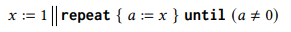
\includegraphics{INF_LOOP_EX1.png}
      }
      \end{figure}

      \begin{itemize}
        \item Under thread fairness, both threads will be scheduled, thus ensuring forward progress. 
        \item However, the loop will not terminate until the corresponding thread can observe the modified write value. 
        \item The loop thread will not terminate until the thread modifying the value of $x$ flushes its write buffer to main memory.
      \end{itemize}
    \end{frame}

    \begin{frame}{New Fairness Requirement}
      
      \begin{center}
        Models of Concurrency must also ensure \emph{Memory Fairness}: That each write is eventually propagated to other threads in any execution. 
      \end{center}

    \end{frame}

    \begin{frame}{Memory Fairness: Layman Terms}
      
      Memory propagation are named Silent Transitions  
      \begin{itemize}
        \item A write memory event is eventually followed by a silent transition to propagate to other threads - Continuously Enabled Silent Transitions.
        \item Every silent transition step exists in any trace execution, and it is followed by the corresponding write event - Memory Fair. 
      \end{itemize}
      
      \begin{center}
        The concrete details on Silent Transition is dependent on the model of concurrency considered.   
      \end{center}
      
    \end{frame}

    \begin{frame}{Towards Memory Fairness Constraint: Key Idea}

      \begin{itemize}
        \item Each memory location will have a total order $\mo$ on the writes which modify them in any concurrent execution (Coherence base).
        \item Each thread must broadcast its write value to other threads, thus ensuring the write is part of the above mentioned total order.
        \item There cannot be infinite writes - $\mo$ finite 
        \item A terminating thread, relying on a shared memory write value cannot perpetually read its stale contents.
        \item Eventually, the reads will read from the latest write in memory - $\rf^{-1};\mo$ or $\fr$ finite.  
      \end{itemize}
  
    \end{frame}

    \begin{frame}{Memory Fairness: Example1}
      
      \begin{figure}
        \makebox[\textwidth][c]{
            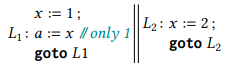
\includegraphics{INF_LOOP_EX3.png}
      }
      \end{figure}
      
      \begin{itemize}
        \item The value of $x$ read by LHS thread cannot always be 1.
        \item This is due to the fact that the other thread writes $x=2$ successively. 
        \item How do we specify such a constraint?
      \end{itemize}

    \end{frame}

    \begin{frame}

      \begin{figure}
        \makebox[\textwidth][c]{
            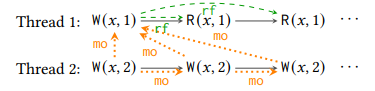
\includegraphics{INF_LOOP_MEM_FAIR_EX3.png}
      }
      \end{figure}

      \begin{itemize}
        \item It cannot be possible that all writes $x=2$ done by the other thread precede the write $x=1$.
        \item Having this would imply $x=1$ perpetually waits for every write done by the other thread to finish. 
        \item A thread cannot wait forever to broadcast its write to other threads.
      \end{itemize}

      \begin{center}
        A write cannot have infinitely many $\mo$ predecessors to the same location.
      \end{center}
      
    \end{frame}

    \begin{frame}
      
      \begin{figure}
        \makebox[\textwidth][c]{
            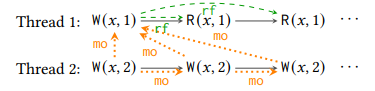
\includegraphics{INF_LOOP_MEM_FAIR_EX3.png}
      }
      \end{figure}

      \begin{itemize}
        \item Lets say every write does broadcast eventually and does not perpetually wait.
        \item Then if there are infinitely many reads, they must eventually read the $\mo$ maximal write value.
        \item A thread must eventually be updated with the latest write value that it can read. 
      \end{itemize}

      \begin{center}
        Every write cannot have infinitely many $\fr$ predecessors to the same location. 
      \end{center}
      
    \end{frame}

    \begin{frame}{Memory Fairness: Example 2}

      \begin{figure}
        \makebox[\textwidth][c]{
            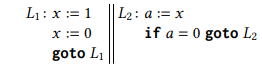
\includegraphics{INF_LOOP_EX2.png}
      }
      \end{figure}

      \begin{itemize}
        \item It is possible in this case for an infinite execution to take place.
        \item LHS thread always finishes broadcasting its write $x=0$ before RHS thread iteration begins.
        \item Such an execution is allowed with the current constraints.
      \end{itemize}

      \begin{itemize}
        \item Each write does not have infinitely many predecessors in $\mo$.
        \item And each write is eventually read, keeping $\fr$ predecessors finite.
      \end{itemize}
      
    \end{frame}

    \begin{frame}{Assumption of Bounded number of Threads}
      \begin{figure}
        \makebox[\textwidth][c]{
            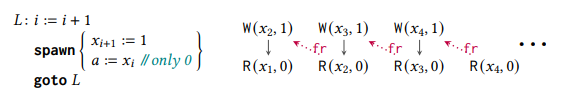
\includegraphics{INF_THREAD_MEM_FAIR_EX5.png}
      }
      \end{figure}

      \begin{itemize}
        \item The $\mo$ and $\fr$ prefix-finiteness is sufficient fairness condition only for bounded number of threads.
        \item The example execution above is not fair: Every read to $x_{i>1}$ must be $1$ instead. 
        \item However, the propagation of writes to the newly spawned thread is not captured by simply pre-fix finiteness of $\mo$ and $\fr$. 
      \end{itemize}

    \end{frame}

    \begin{frame}{Fairness for Weaker Models}

      \begin{itemize}
        \item The declarative style memory fairness conditions for $TSO, RA$, Strong$COH$ and $RC11$ remain the same.
        \item To recap the memory-fairness constraint is $\mo, \fr$ prefix-finiteness.
        \item The above models have $\po \cup \rf$ acyclic as a common constraint in the semantic model.
        \item For models not obeying this constraint, a different fairness constraint is required.
      \end{itemize}
      
      \begin{center}
        The compilation correctness and optimization safety guarantees for $RC11$ remain unchanged on adding the fairness constraint.
      \end{center}

    \end{frame}


    \begin{frame}{Limitation and Future Work}

      \begin{itemize}
        \item Fairness assuming bounded number of threads.
        \item Fairness constraint identified for models respecting $\po \cup \rf$ acyclicity constraint.
        \item Not clear the proposed fairness constraint of prefix-finiteness is for \textbf{all models respecting $\po \cup \rf$ acyclicity constraint}. 
      \end{itemize}
      
    \end{frame}

    \begin{frame}{Further to Read in Paper}

      \begin{itemize}
        \item The operational memory-fairness constraints for discussed models.
        \item Reasoning about termination of different lock implementations using declarative models and the new memory fairness constraint.
        \item Proof of preserving compilation and optimization safety of $RC11$ on adding memory fairness constraint.
        \item Preservation of Robustness Guarantees across all models considered in paper.
      \end{itemize}
      
    \end{frame}

    \begin{frame}{Thank you}

      Questions?
      
    \end{frame}


  \end{document}